\chapter{Evaluation} \label{chap:system_archi}
This chapter describes the evaluation method and metrics used to measure the performance of the models. Additionally to validate the results of the Machine Learning models, a semi-structured interview conducted with the members of the marketing and sales team validates the significance of the approach used in this work. 
\section{Methods} \label{sect:thefirst}
To measure the performance of a machine learning based application there are certain metrics defined which indicates how well the the machine learning model has been trained. For example in a image classification problem, evaluation metrics such as precision, recall, F1 score, accuracy are used to denote how well the application can recognise a particular image. Similarly, there are some evaluation metrics defined that can be utilized to measure the performance of machine learning based recommender system. Furthermore such metrics also aid in selecting the appropriate algorithm.  \\ \par


The most common evaluation strategy used when deploying the recommender system in real-world environment consist of two methods namely: Online evaluation and Offline Evaluation.
\begin{itemize}
	\item \textit{Online Evaluation}\\
	 It helps in measuring the performance of the recommender system in real-life situations where the users interact with the system. One such way of implementing online evaluation is through A/B testing. Typically, A/B testing involves serving a fraction of random users with recommendations generated from recommender system A and another fraction with recommender system B. A utility function such as Click Through Rate (CTR) is then used which indicates which recommender system is more successful in attracting the user or capturing his interest. The results from such experiments helps in further fine tuning the algorithm to obtain the desired level of performance. Although Online evaluation techniques are useful, they require meticulous planning. Moreover, the cost associated with conducting such experiments are usually high owing to the significant investment in terms of resources, money and time \autocite[2941]{gunawardana2009survey}. Implementing an Online Evaluation experiments is out of scope of this study and hence has been excluded.
	\item \textit{Offline Evaluation}
	In most of the cases Online Evaluation is followed after Offline evaluation process. This is mainly because of the costs associated with Online Evaluation as well as to avoid any undesirable experience for the users of the system. Offline Evaluation provides the necessary experimentation setup for implementing different algorithm and testing it to achieve the desired level of performance. Recently there has been tremendous development in the algorithms for recommender systems suitable for a particular task. Offline evaluation setup exclude other algorithms and retain only those which showcase promising results which can be further extended to the Online evaluation phase thus reducing the risk of failure in later stages \autocite[2941]{gunawardana2009survey}. Offline evaluation tries to mimic the real-world environment by using the user-item interaction data-set similar to that of real-world deployment. In most of the scenarios the user-item interaction data-set refers to the past transactions, historical data related to the user,items and ratings. Depending on the underlying task of the recommender system i.e either to predict the ratings for unknown items for user or recommendations, the approach for training the machine learning model changes. In traditional machine learning problem, the data-set is divided into training data and testing data, where patterns are learned from the training set and are evaluated on the testing set. In recommender system following similar approach will lead to creating a bias, as some part of the data-set is not used leading to incorrect learning patters. One such strategy especially adopted while training machine learning models used in recommender systems is to mask certain percentage of the user-item interaction data to create the training data-set while the original data-set can be used as the testing data-set.
	
\end{itemize}


Since the development of recommender system is influenced by the underlying tasks such as Ratings Prediction, Recommending Good items, or Optimizing some utility function \autocite[2938]{gunawardana2009survey}, the selection of the evaluation metric is specific to the task. The following section elaborates more on the metrics used specifically for recommender systems.

\section{Metrics}
As mentioned before the typical task associated with recommender system is either to Predict the ratings or to recommend some items. When evaluating recommender system the choice of evaluation metric is also dependent on factors such as the expected tasks, type of data (implicit or explicit) that is available for learning the machine learning models. As a result not all metrics can be used to measure the performance of the algorithm. Literature suggests that the metrics can be broadly divided into three categories Error based metrics, Accuracy based metrics, and Ranking based metrics as seen in table \ref{table:1}.  \\

\begin{table}[h!]
\centering
\begin{tabular}{|c| c| c|} 
 \hline 
 No. & Metric & Category\\ [0.5ex] 
 \hline \hline
 1 & Root Mean Squared Error (RMSE) & Error based \\ 
 \hline
 2 & Mean Squared Error (MSE) & Error based \\ 
 \hline
 3 & Mean Absolute Error (MAE) & Error based \\ 
 \hline
 4 & Mean Average Precision (MAP) & Accuracy based \\ 
 \hline
 5 & Mean Average Recall (MAR) & Accuracy based \\
 \hline
 6 & Mean Reciprocal Rank (MRR)  & Rank based \\ 
 \hline
 7 & Normalized Discounted Cumulative Gain (NDGC) & Rank based \\ 
 \hline
\end{tabular}
\caption{Categorization of evaluation metrics}
\label{table:1}
\end{table}

\begin{itemize}
	\item \textit{Error based metrics}: Typically used when a rich data-set containing explicit ratings for items is available and we want to predict the ratings for the items which were not rated by the user. Metrics such as Root Mean Squared Error (RMSE), Mean Squared Error (MSE), Mean Absolute Error(MAE) are often used in such scenario. 
	\item \textit{Accuracy based metrics}: These metrics are useful in determining the relevancy of the recommendations generated for the users. Inspiration on the usage of such metrics is drawn from the Information Retrieval domain, where the objective is to retrieve information within documents or retrieving relevant documents to a given query. Similarly, in recommender systems given the set of interactions between users and items, the recommender system should be able to recommend items that may be relevant to the user. Using this understanding, we can construct the basic structure for the evaluation. One such construct is \textit{confusion matrix} as show in Fig \ref{fig:confusion_matrix}, where each row in the matrix represents the outcome of the recommender system and the columns represent the actual observed interaction between user and item. Since this study is based on implicit feedback data represented in binary format i.e. if a user preferred an item or not, accuracy based evaluation metrics are more suitable for evaluating algorithm performance. Some of the most commonly used metrics are Mean Average Precision (MAP@K), Mean Average Recall(MRR@K).
	
	\item \textit{Rank based metrics}: Such metrics are used when the ranking is of importance in the top-k results generated by the recommender system. The most commonly used metrics are Normalized Discounted Cumulative Gain (NDGC), Mean Reciprocal Rank (MRR)
\end{itemize} 
\\ \par

The metrics that have been used to evaluated the machine learning models in this study are briefly described below.RMSE is one of the popular method used for evaluating an algorithm. The equation for calculating MSE and RMSE is given in Equation \ref{eqn:MSE} and Equation \ref{eqn:RMSE} respectively. The smaller the difference between the predicted and the actual value, the better is the performance of the algorithm. 

\begin{equation}
\label{eqn:MSE}MSE =  \frac{1}{N}\sum_{i=1}^{N} (x_{i,j}-y_{i,j})^2
\end{equation}
\\
\begin{equation}
\label{eqn:RMSE}RMSE = \sqrt{ \frac{1}{N}\sum_{i=1}^{N} (x_{i,j}-y_{i,j})^2}
\end{equation}

where N is the number of users and x{\_i,j} represents the predicted rating and y{\_i,j} represents the actual rating. \\ \par

For calculating the accuracy based metrics, the \textit{confusion matrix} is referred as it keeps track of the number of times the recommendation falls into one of the 







\begin{figure}
    \centering
    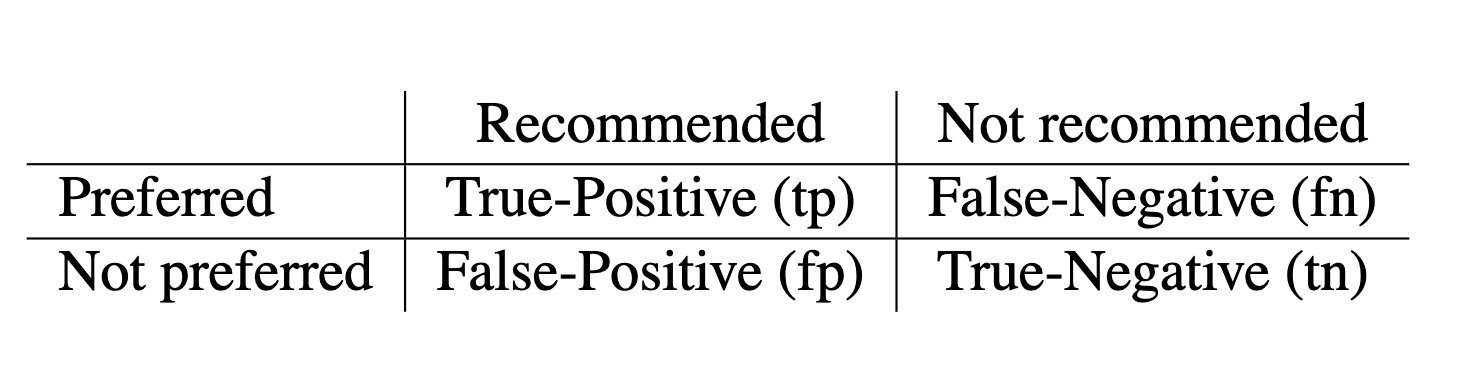
\includegraphics[scale=0.5]{chapters/figures/confusion_matrix.png}
    \caption{Representation of Recommender System result in the form of Confusion Matrix \autocite[2945]{gunawardana2009survey}}
    \label{fig:confusion_matrix}
\end{figure}


\section{Qualitative Interviews}

\subsection{Interview Guideline and Choice of Interview Partners}
\subsection{Overview of Interview Conducted}
\section{Qualitative Content Analysis of the Interviews}

